\section{Results}\label{sec:results}

\begin{figure*}
    \begin{center}
        %\hspace{-7mm}
        % fig 1, 4-14
        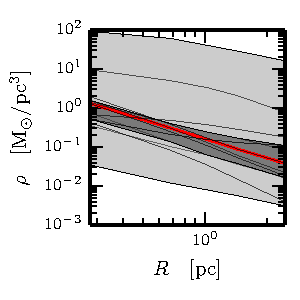
\includegraphics[width=0.33\textwidth]{fig/fornax/prof_rho_0}
        \includegraphics[width=0.33\textwidth]{fig/fornax/prof_nr_0}
        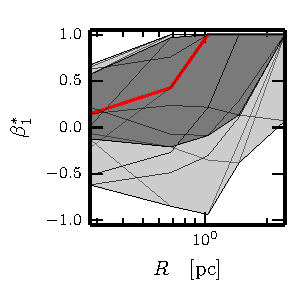
\includegraphics[width=0.33\textwidth]{fig/fornax/prof_betastar_1}
        % TODO: look up analytic beta profile, looks like there is a 1/r_scale bug
        \caption{Reconstructed density, density slope, and velocity
          anisotropy of Fornax (red shows median, shaded areas
          show the 68 and 95 percentiles) for TODO tracer particles, after
          TODO iterations. The vertical lines give the projected
          half-light radius (for 2D quantities), and the half-light
          radius for the median model for 3D quantities.}
        \label{fig:fornax}
    \end{center}
\end{figure*}

TODO: $chi^2$ distribution, Sigma, sigma


\begin{figure*}
    \begin{center}
        %\hspace{-7mm}
        % fig 1, 4-14
        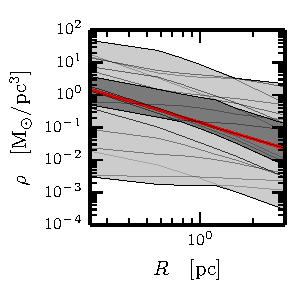
\includegraphics[width=0.33\textwidth]{fig/carina/prof_rho_0}
        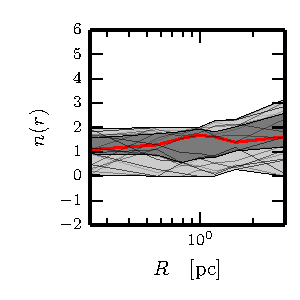
\includegraphics[width=0.33\textwidth]{fig/carina/prof_nr_0}
        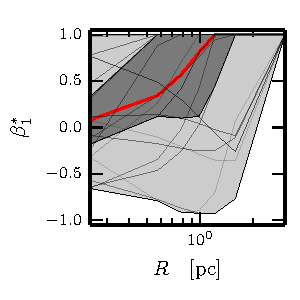
\includegraphics[width=0.33\textwidth]{fig/carina/prof_betastar_1}
        % TODO: look up analytic beta profile, looks like there is a 1/r_scale bug
        \caption{Reconstructed density, density slope, and velocity
          anisotropy of Carina (red shows median, shaded areas
          show the 68 and 95 percentiles) for TODO tracer particles, after
          TODO iterations. The vertical lines give the projected
          half-light radius (for 2D quantities), and the half-light
          radius for the median model for 3D quantities.}
        \label{fig:fornax}
    \end{center}
\end{figure*}

\begin{figure*}
    \begin{center}
        %\hspace{-7mm}
        % fig 1, 4-14
        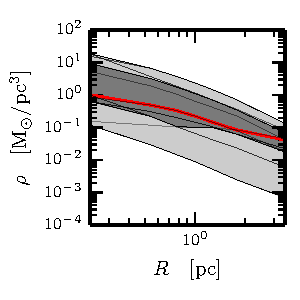
\includegraphics[width=0.33\textwidth]{fig/sculptor/prof_rho_0}
        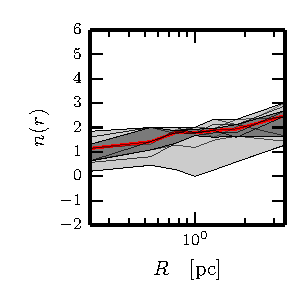
\includegraphics[width=0.33\textwidth]{fig/sculptor/prof_nr_0}
        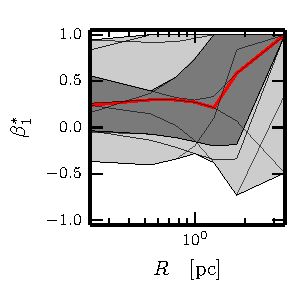
\includegraphics[width=0.33\textwidth]{fig/sculptor/prof_betastar_1}
        % TODO: look up analytic beta profile, looks like there is a 1/r_scale bug
        \caption{Reconstructed density, density slope, and velocity
          anisotropy of Sculptor (red shows median, shaded areas
          show the 68 and 95 percentiles) for TODO tracer particles, after
          TODO iterations. The vertical lines give the projected
          half-light radius (for 2D quantities), and the half-light
          radius for the median model for 3D quantities.}
        \label{fig:fornax}
    \end{center}
\end{figure*}

TODO: Sextans
%\begin{figure*}
%    \begin{center}
%        %\hspace{-7mm}
%        % fig 1, 4-14
%        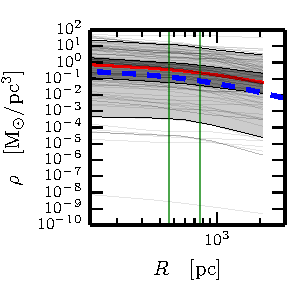
\includegraphics[width=0.4\textwidth]{fig/sextans/prof_rho_0.pdf}
%        \includegraphics[width=0.4\textwidth]{fig/sextans/prof_nr_0.pdf}
%        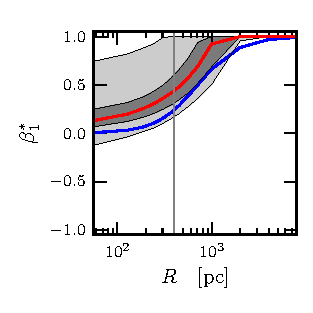
\includegraphics[width=0.4\textwidth]{fig/sextans/prof_betastar_1.pdf}
%        % TODO: look up analytic beta profile, looks like there is a 1/r_scale bug
%        \caption{Reconstructed density, density slope, and velocity
%          anisotropy of Sextans (red shows median, shaded areas
%          show the 68 and 95 percentiles) for TODO tracer particles, after
%          TODO iterations. The vertical lines give the projected
%          half-light radius (for 2D quantities), and the half-light
%          radius for the median model for 3D quantities.}
%        \label{fig:fornax}
%    \end{center}
%\end{figure*}






%%% Local Variables: 
%%% mode: latex
%%% TeX-master: "Steger+_2014_Gravlite"
%%% End: 
